\chapter{Laboratorio 1}
Il primo circuito realizzato in laboratorio è un \textit{emmitter follower}, di cui si riporta di seguito lo schematico:
\begin{figure}[h!]
	\centering
	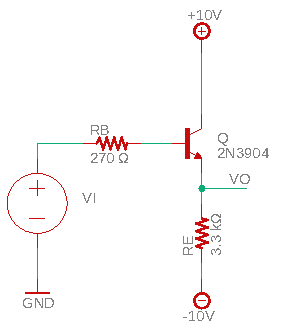
\includegraphics[width=0.4\linewidth]{./OtherFiles/Laboratorio 1/emitter follower}
	\caption{Schematico del circuito emitter follower.}
	\label{fig:emitterfollwer}
\end{figure}
\section{Punto di lavoro}
Per analizzare il circuito, si procede all'analisi del punto di lavoro, dove i generatori di tensioni e correnti alternate vengono sostituiti rispettivamente con un corto circuito o un circuito aperto.
\begin{figure}[h!]
	\centering
	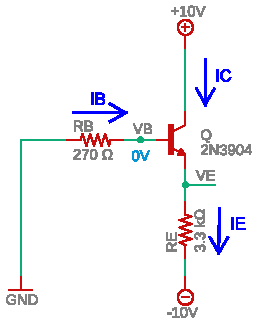
\includegraphics[width=0.4\linewidth]{./OtherFiles/Laboratorio 1/emitter follower_punto di lavoro_printout}
	\caption{Analisi del punto di lavoro del circuito emitter follower.}
	\label{fig:emitterfollwer_puntodilavoro}
\end{figure}
In particolare, il generatore di tensione (di segnale) V\textsubscript{in} viene quindi considerato come un corto circuito che collega un terminale della resistenza R\textsubscript{B} a massa. Considerando il modello ideale del transistor Q , con $\beta\overrightarrow{}\infty$ e corrente di base nulla, si ricava che la corrente che attraversa la resistenza R\textsubscript{B} è nulla. Per cui, per la legge di Ohm $V=R*I$, la caduta di potenziale sulla resistenza è nulla. Per cui il nodo V\textsubscript{B} si trova a una tensione di \SI{0}{\volt}. 

Se si esegue un bilancio di correnti delle correnti uscenti e entranti nel transistor si ottiene $I\sub{B}+I\sub{C}=I\sub{E}$. Dal momento che la corrente I\sub{B} è nulla, I\sub{C} = I\sub{E}.

Supponendo che il transistor si trovi in regione attiva diretta, $V\sub{BE}=+\SI{0.7}{\volt}$. Quindi, $V_E=V_B-\SI{0.7}{\volt}= -\SI{0.7}{\volt}$.

Infine, la corrente di emettitore (e di conseguenza anche la corrente di collettore) si ricava dalla legge di Ohm: $I_E=I_C=\frac{\Delta V}{R_E}=\frac{V_E-(-\SI{10}{\volt})}{R_E}$. 

Come si può notare, si verifica l'ipotesi che il transistor si trova in regione attiva diretta, dal momento che $V_{CB}>0$.

Avendo ricavato la corrente di collettore stazionaria, è utile calcolare anche la transcoduttanza del transistor: $g_m=\frac{I_C^*}{\phi_T}$. Essa sarà utile nell'analisi di piccolo segnale.
\section{Analisi di piccolo segnale}
\begin{figure}[h!]
	\centering
	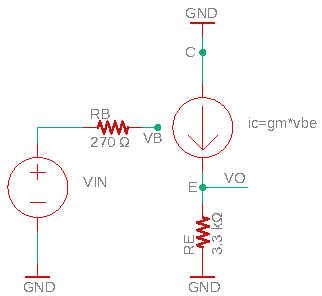
\includegraphics[width=0.4\linewidth]{./OtherFiles/Laboratorio 1/emitter follower_piccolo segnale}
	\caption{Analisi di piccolo segnale del circuito emitter follower.}
	\label{fig:emitterfollwer_piccolo segnale}
\end{figure}
\section{Componenti e misure}
\begin{figure}[h!]
	\centering
	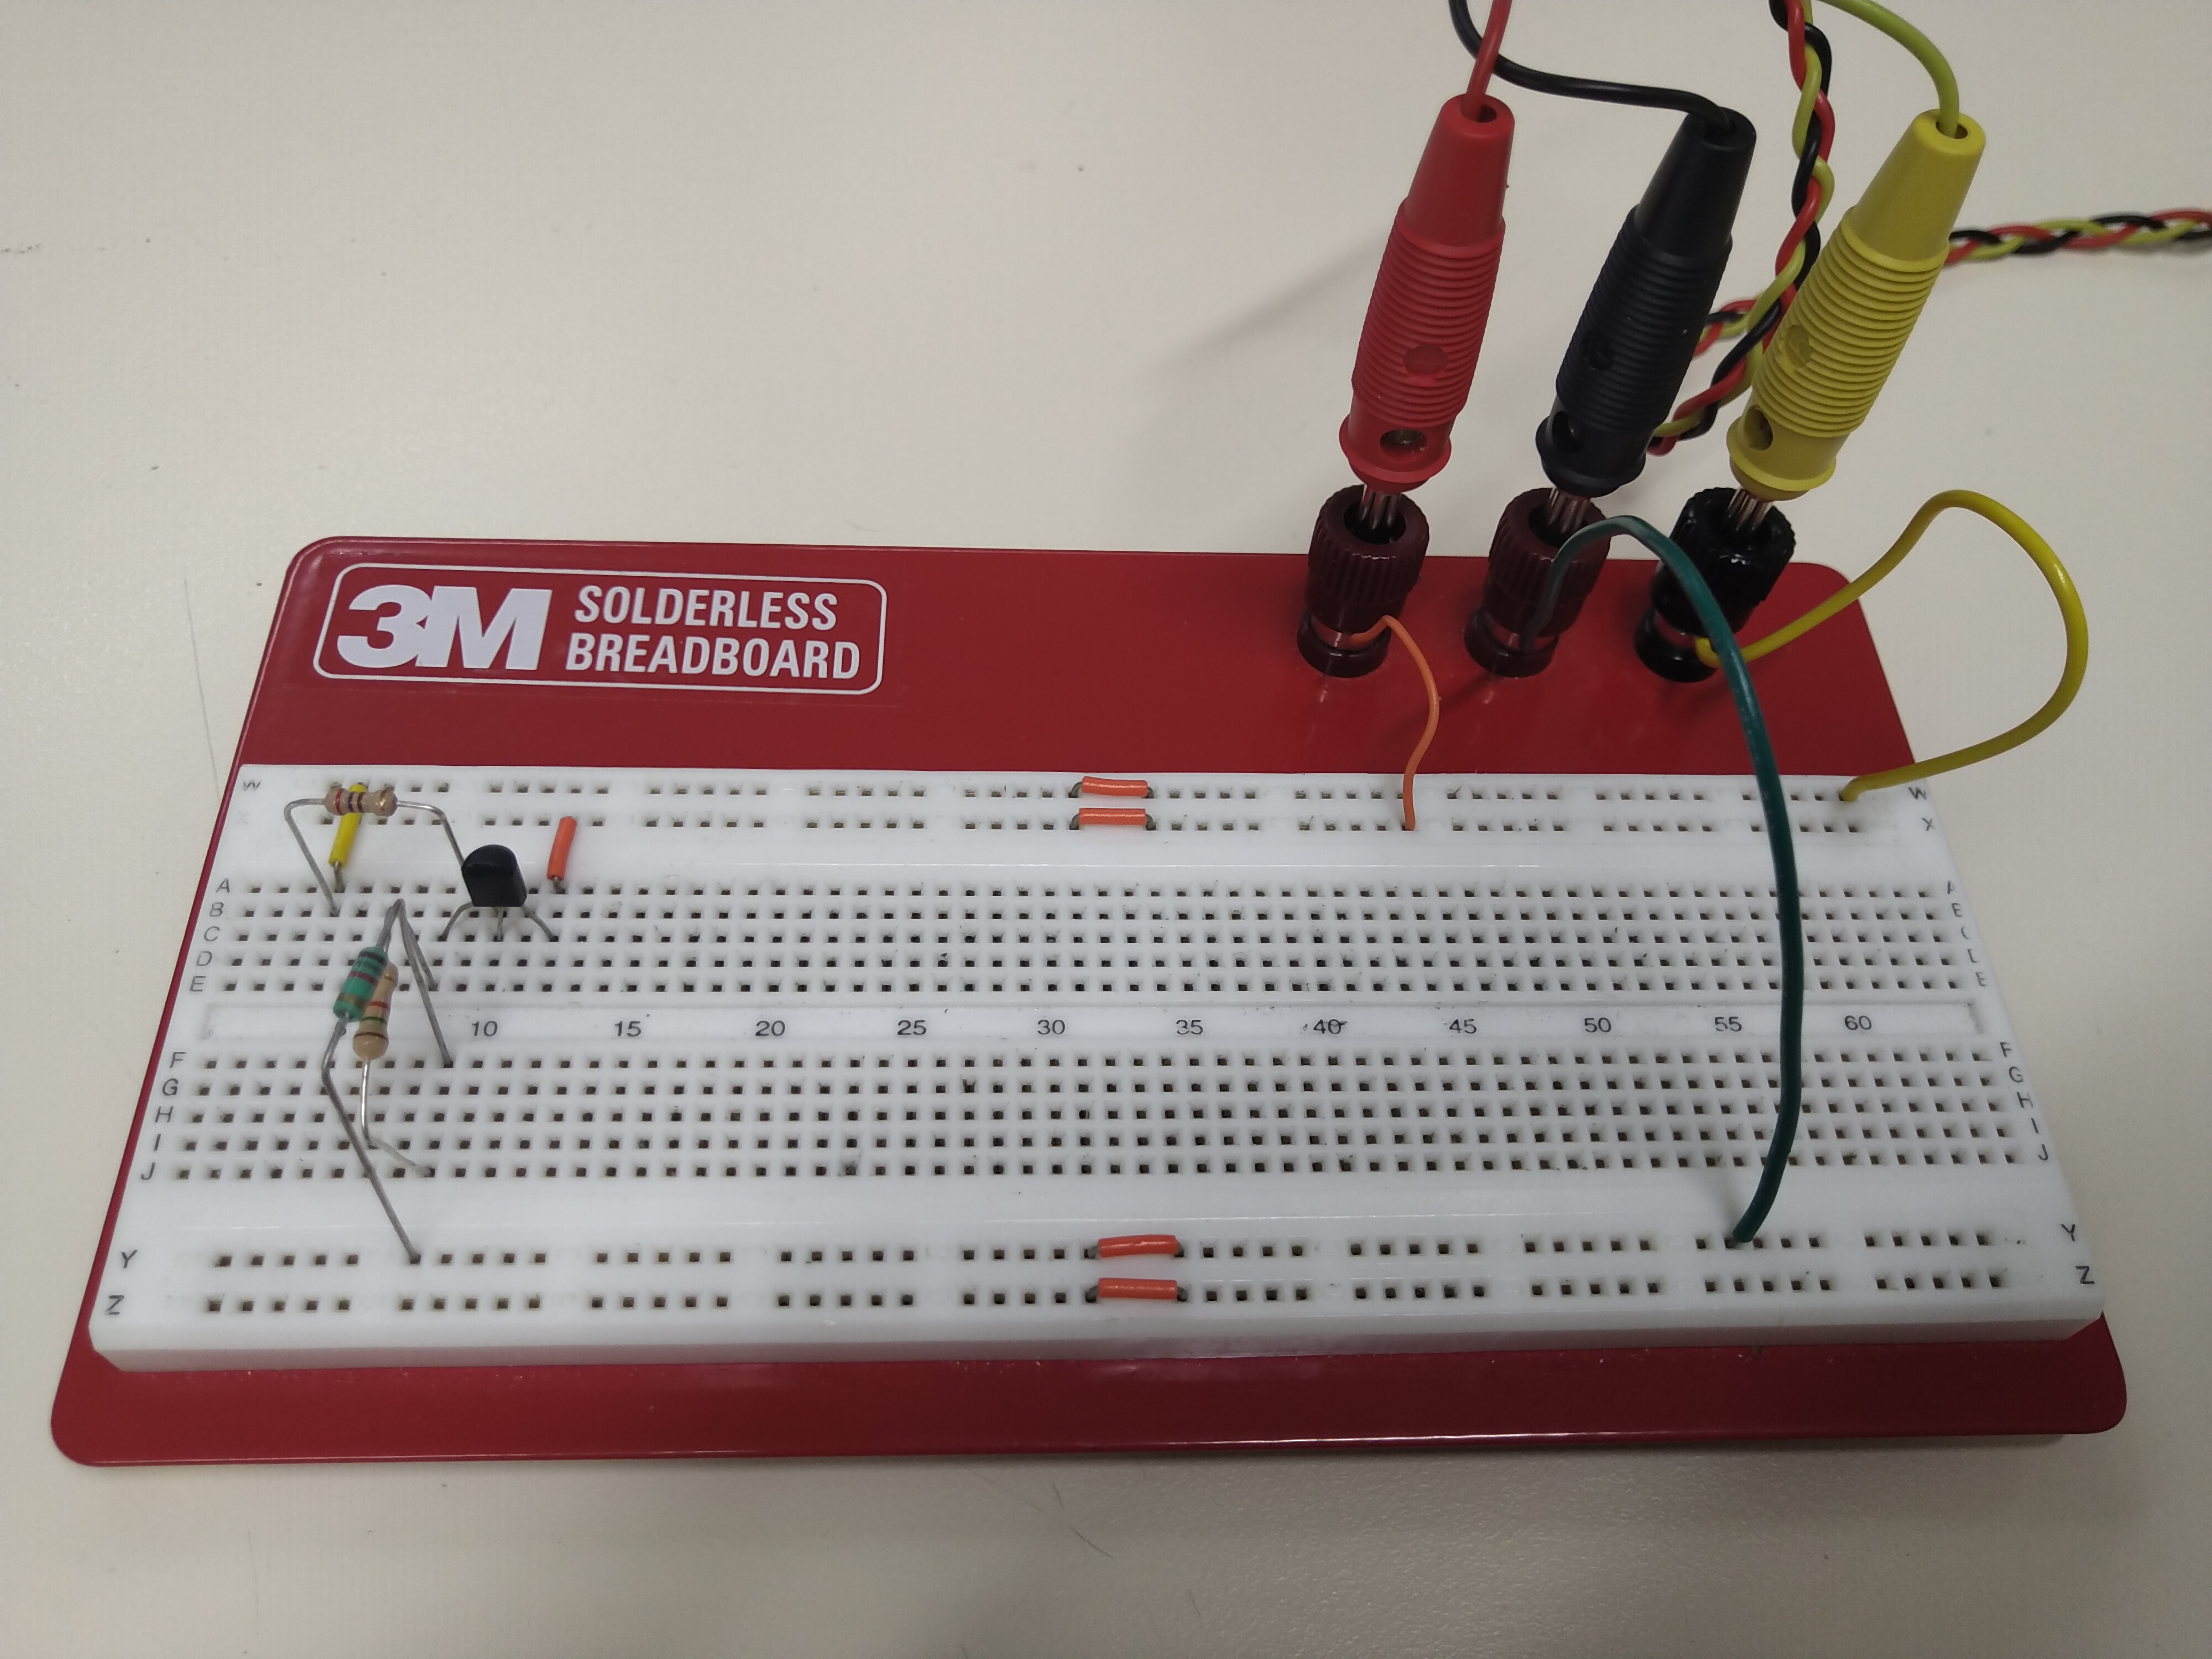
\includegraphics[width=0.4\linewidth]{./ImageFiles/Laboratorio 1/IMG_20220510_103526}
	\caption{Foto del circuito realizzato in laboratorio.}
	\label{fig:emitterfollwer_circuito}
\end{figure}